
\chapter{Mixed Precision Bounding Volume Hierarchy}\label{ch:simd_bvh}

\section{Introduction}

As established in Section \ref{sec:problem-statement}, the dominant source of
additional runtime in DAGMC is spent in the ray tracing process used to satisfy
the Monte Carlo geometry queries outlined in Section \ref{sec:mc-geom-queries}.
The focus of the work in this chapter is improvements on the performance of the
ray tracing process through the application of SIMD-oriented programming in the
bounding volume hierarchies used in DAGMC. Some preliminary work was performed
in this area by replacing the ray tracing kernel used in DAGMC (MOAB's oriented
bounding box tree) with a kernel produced by Intel, called Embree.

\section{Linking DAGMC with Intel's Embree}\label{sec:embree}

Embree is the result of a an effort to produce a performant CPU-based ray tracer
as a demonstration of the expanding capabilities of modern CPU architectures
\cite{Wald_2014}. In both construction and traversal of BVHs, Embree takes
advantage of many of the latest developments in BVH research by using modern
chipset architecture capabilities via vectorization at an implementation level
as described in Section \ref{subsec:arch} of this work. The combination of these
effects leads to a very powerful ray tracing tool in terms of performance, as
demonstrated by the many projects which have incorporated Embree as their
production ray tracing kernel such as Corona, Autodesk, FluidRay, and
Brighter3D. As a result of its success in other areas, Embree was selected to be
applied in DAGMC to satisfy geometric queries for MCNP. The resulting
combination of these tools will be referred to as EmDAG.

\subsection{Implementation and Model Transfer}\label{sec:emdag_transfer}

The process of employing Embree as DAGMC's ray tracer begins by establishing an
equivalent representation of the MOAB mesh in Embree. In comparison to MOAB,
Embree is limited in its ability to represent the underlying topological
structure of a model. This topology is necessary and used advantageously during
particle tracking in DAGMC by reducing the set of triangles queried to those of
the particle's current volume and thus reducing the number of point containment
queries. However, a method was discovered to represent enough of the topology to
meet the requirements of DAGMC transport. The highest level representation in
Embree is referred to as a scene. Each scene may contain one or more geometries
or triangle surface meshes. Fortunately, this system is enough to create a
workable representation of DAGMC meshes in which MOAB volumes are the equivalent
of Embree scenes and MOAB surfaces are represented in their respective scenes as
surfaces. This method provides a one-to-one mapping of MOAB volumes and surfaces
to their corresponding entities in Embree and allows all topology-based
operations to proceed inside of DAGMC in their usual manner. In this way, the
requirement for topological information in DAGMC at the surface and volume level
is met. Next, transfer of the primitive mesh data is considered.

Scenes do not share mesh data as volumes are able to do in MOAB, so the triangle
connectivity of each surface is reproduced in each scene they belong
to. Fortunately, Embree does allow the sharing of vertices between scenes. In
order to take advantage of this feature, all of the vertices in the MOAB mesh
are provided in the Embree instance as a global vertex buffer. Surfaces from all
scenes can then be defined by a connectivity of vertices from this global pool
of points. This method guarantees that the each surface can be represented by
the same set of stored vertices in each scene it belongs to giving the exact
same representation in each scene. It greatly simplifies particle tracking by
guaranteeing that the same surfaces will not overlap each other in the different
scenes they are a part of by doing the conversion of points from the MOAB
database to Embree only once. Additionally, this method will maintain
watertightness at the boundaries between surfaces ensuring the same model
fidelity as the representation in MOAB.

\begin{figure}
  \centering
  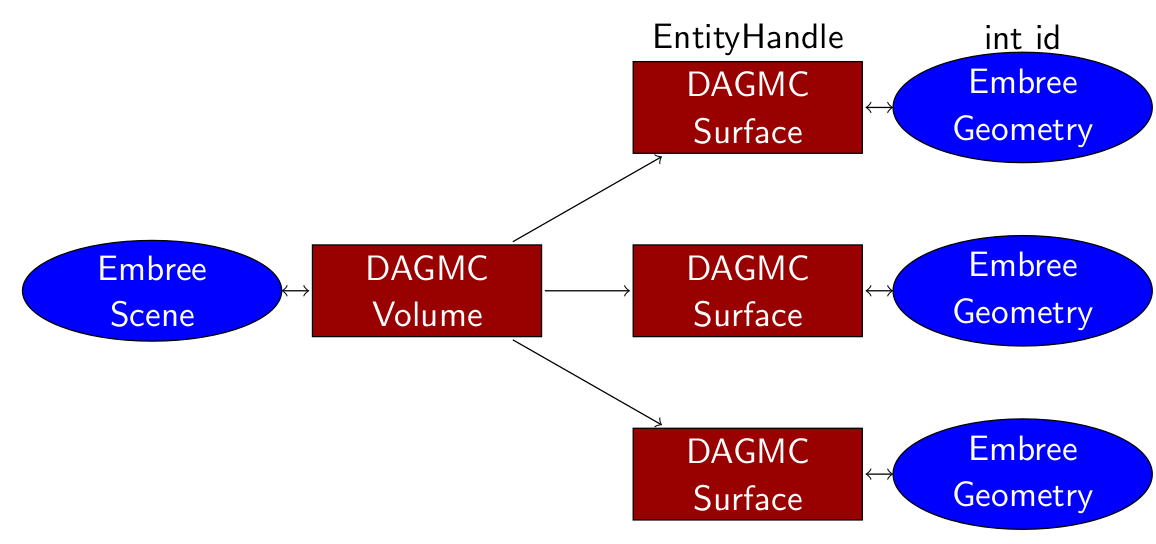
\includegraphics[scale=0.3]{emdag_mapping.png}
  \caption{Representation of MOAB tracking topological connections while mapped
    to Embree to perform ray queries.}
  \label{emdag_mapping}
\end{figure}

The representation of triangle normals are important to the DAGMC particle
tracking algorithm established by Smith et. al. in 2011 \cite{Smith_2011}. In
DAGMC, particles on or just outside the surface of a volume are handled by
ignoring the near-surface intersection upon being established in a new
volume. This is done to maintain tracking of particles based on their logical
position in the model rather than solely their numerical position which can
cause ambiguities regarding point containment and cause lost particles or
trapped particles between surfaces with infinite histories. Logical particle
tracking is implemented using the convention that triangle normals will always
point outward from the center of the volume they belong to. Triangles hit by the
ray are ignored if the normal of the triangle opposes the ray direction via a
dot product calculation to ensure only exiting ray intersections are
considered. While this has historically been handled inside of DAGMC, this is
accomplished in EmDAG via the use of Embree's filter functions. Filter functions
allow for a user-defined callback method which allows users to validate a ray
hit inside of Embree before returning a final result. Embree will return its
most recent intersection with the scene to the filter function (the hit
triangle's unnormalized vector included) and allow a method to either accept the
hit or instruct Embree to continue tracing the ray path based on the outcome of
the filter function. In MOAB, triangle normals are set in a global manner and
adjusted using stored information within MOAB based on what volume is being
queried at the moment. This is referred to as the surface's sense with respect
to that volume. Because we are forced to duplicate surfaces in Embree, the
triangle normals are pre-oriented based on this surface's sense for the scene it
is being created in upon initialization of the model within the Embree
instance. This saves steps in gathering this information upon traversal when the
triangle normal is needed to determine a particle's logical position within the
model. Though the connectivity of triangles is duplicated using this approach,
the overall memory footprint of EmDAG after duplicating the DAGMC geometry in
Embree is not much greater thanks to the single precision values for vertex
locations used in Embree which will be addressed in a later section of this
chapter.  By meeting DAGMC's requirements in the areas of topology, watertight
representation, and hit acceptance/rejection based on triangle normals, Embree
provides DAGMC with all the information needed to perform geometric operations
required by the various Monte Carlo codes it supports, but in an agnostic manner
to the ray tracing kernel being used.

\subsection{Ray Fire Performance}\label{subsubsec:emdag_rf_performance}

Using the same DAGMC-based ray fire test program, the performance of DAGMC's ray
fire ability was compared to that of EmDAG's for three models. These models
include a simple sphere, a notched sphere, and a high aspect ratio (HAR)
cylinder. In each of these tests, the models are tessellated with an
increasingly smaller faceting tolerance in a higher number of triangles and more
complex nature of the surface mesh in terms of BVH construction and
traversal. The faceting tolerance is defined as the maximum distance between the
faceted curve or surface and the geometric curve or surface which it
resolves. 600k rays are then fired from the center of the volume isotropically
using the same random number seed so that the same set of rays is fired in each
ray tracing system.

\begin{figure}[H]
  \begin{center}
    \begin{tabular}{ccc}
      \includegraphics[scale=0.15]{sphere.eps} &
      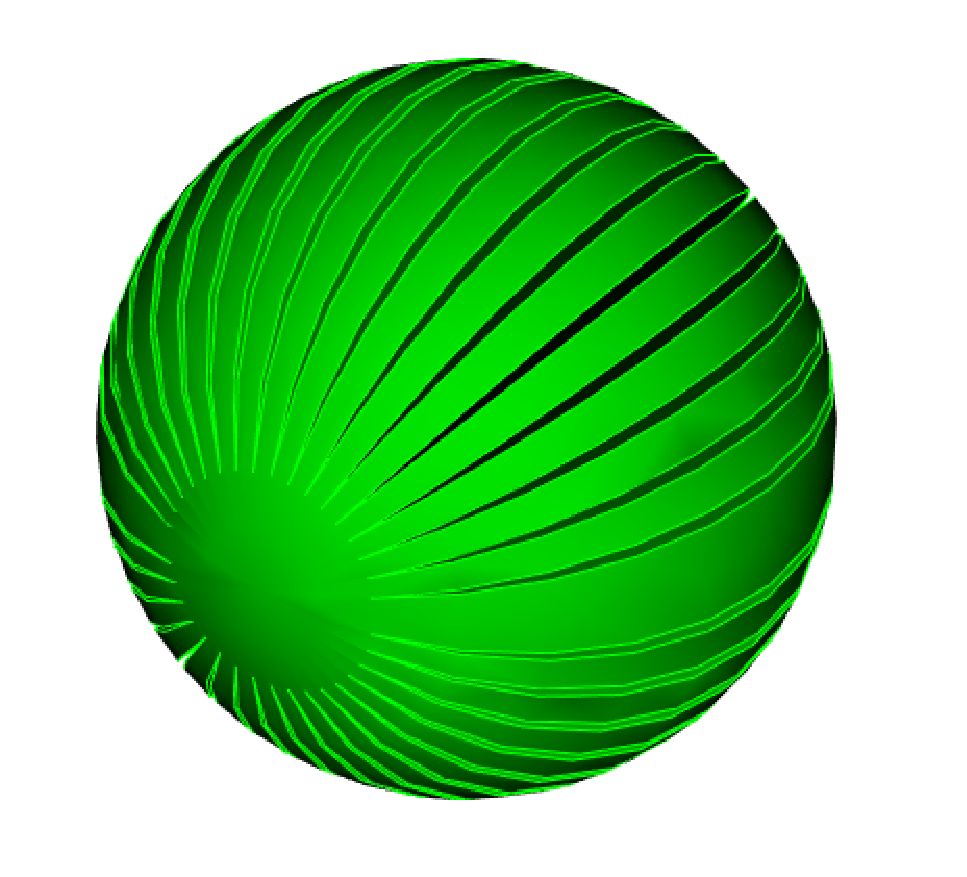
\includegraphics[scale=0.15]{ds.eps} &
      \includegraphics[scale=0.15]{larcyl.eps} \\
    \end{tabular}
    \caption{CAD representations of the sphere, slotted sphere, and high aspect
      ratio cylinder test models used for ray fire timings of DAGMC and
      EmDAGMC. (left to right) \label{models}}
  \end{center}
\end{figure} 

The sphere and slotted sphere models present specialized challenges to the BVH
data structure as described in Section \ref{sec:hv_study_MOAB}. Due to memory constraints
of the system used for testing EmDAG's performance against DAGMC, the ITER
volume was removed and replaced with a high aspect ratio cylinder. The faceting
of the cylinder contains many long, thin triangles running along the barrel of
the cylinder. In similar fashion to the spherical model, the number of these
triangles will increase with decreasing faceting tolerance resulting in an
increasing triangle density as well. The low aspect ratio nature of these
triangles can cause difficulty in the calculations of tightly fitting OBBs
within MOAB's BVH builder. This test model is used to the ray tracing systems
robustness of the BVH generation algorithms to objects with surface meshes of
this nature.

The standard DAGMC ray fire test program (included in appendix A) was used to
evaluate both ray fire systems. The test program itself is agnostic to the
underlying ray tracing kernel used by DAGMC and two versions of the program were
compiled. One in which DAGMC uses MOAB's ray tracer and another in which MOAB's
ray tracing system is subverted by Embree, a.k.a. EmDAG. The two sets of timing
results can be found in Figure \ref{emdag_timing_compare}.

\begin{figure}[H]
  \vspace{-3cm}
  \centering

  \begin{minipage}{.5\textwidth}
    \centering
    \includegraphics[scale=0.35]{Eig_fix_rf.eps}
  \end{minipage}%
  \begin{minipage}{.5\textwidth}
    \centering
    \includegraphics[scale=0.35]{embree_rf.eps}
  \end{minipage}
  \caption{A comparison of average ray fire times between DAGMC using MOAB's ray
    tracing and Embree. Please note the difference in time scale.}
  \label{emdag_timing_compare}
\end{figure}

Both MOAB and EmDAG scale relatively well for the HAR cylinder model with
decreasing faceting tolerance. This indicates that both systems are capable of
building bounding volumes well for a model with long, skinny triangles. The
scaling of the spherical case with increasing triangles is slightly worse than
the HAR cylinder most likely because the BVH tree is unavoidably going to
become gradually deeper as more and more triangles exist in the model. Finally,
the slotted sphere contains many high valence regions and as expected it scales
the worst with decreasing faceting tolerance as the valence of these regions
increases. It is very apparent that there is nearly an order of magnitude
difference in the ray fire timings MOAB and Embree. Due to the very similar
scaling of each test model, it can be stated that the majority of the
discrepancy in the ray fire timings between the two systems occurs in the
traversal methods employed by both systems and isn't likely due to a significant
difference in the structure of the BVH being built by either system. Changes in
the way the BVH is built typically accounts for anywhere from 30-40\% difference
in ray fire timings whereas the discrepancy seen here between MOAB and Embree is
on average \textbf{an order of magnitude better} when using Embree. In large
part, this has to do with Embree's freedom of design without the restriction of
a ray tracing implementation inside the context of another application. MOAB's
flexibility in core design allows for the robust implementation of an oriented
bounding box tree within this context, but comes with the overhead of database
calls to retrieve stored information which can be undesirable for a
high-performance system and doesn't allow MOAB to take advantage of some
implementation optimization that Embree does. The vectorization of Embree's
traversal through its BVH contributes greatly to its speed. This can be also
considered a part of the design freedom allowed when designing an independent
ray tracing system that cannot not be afforded using only MOAB's database
interface. However, a property unique to MOAB may allow for an implementation
such as this as will be discussed near the end of this work.

\subsection{Transport Tests}
\label{subsec:emdag_transport}

As an extension of these pure ray fire tests, the effect of an improved ray
tracing system on particle transport was studied as well. These tests begin with
several simple models and end with the application of EmDAG to one of the models
used for DAGMC performance benchmarking in Chapter \ref{ch:introduction}, FNG.

The first transport models to be tested were a single cube and single sphere
filled with a dense hydrogen material for high collisionality in the problem
resulting in a large number of ray queries in the transport run. Each of these
models' principal dimension is 10 cm. The source for these models is a 5 MeV
neutron isotropic point source at the center of the volume. One million
particles were simulated in each test. All of the test models were preprocessed
using a faceting tolerance of $10^{-4}$cm. Moving upward in complexity, another
set of tests were run using a set of nested cubes and nested spheres. Each of
the nested volume models contained three cells: the inner volume, a shell
volume, and the graveyard volume. The purpose of these tests was to ensure that
particles could in fact be tracked through multiple volumes robustly. The nested
cubes model contains an extra volume which consists of the original single cube
subtracted from a cube 1cm larger in each dimension. The nested sphere model
contains an extra volume consisting of the original sphere from the single
volume model subtracted from a sphere 1cm larger in radius. As the purpose of
these tests was to test EmDAG's particle tracking between non-zero importance
cells, the dimensions of the offset between the nested volumes is largely
irrelevant so long as particles are in fact reaching all of the cells.

\begin{table}[H]
  \small
  \begin{center}

      \label{timings}
    \begin{tabular}{lccc}

      \toprule
      Test Model & MCNP & DAG-MCNP & EmDAG-MCNP \\
      %%\hline
      & \multicolumn{3}{c}{\textbf{time (min)/ ratio to MCNP}} \\
      \hline
      Sphere & 2.93 / 1.00 & 25.13 / 8.58  & 4.73 / 1.61  \\
      Cube & 5.03 / 1.00 & 10.56 / 2.10 & 5.80 / 1.153 \\
      Nested Spheres & 4.35 / 1.00  & 50.82 / 11.68  & 7.94 / 1.83 \\
      Nested Cubes & 4.73 / 1.00 & 9.26 / 1.96 & 4.35 / 0.92 \\
      \bottomrule
      
    \end{tabular}
  \end{center}
  \caption{Runtime comparison native MCNP, DAG-MCNP, and EmDAG-MCNP over four
    transport test problems.}
  
\end{table}

The native MCNP runs were generally the fastest among the test problems with the
exception of the nested cubes case in which EmDAG-MCNP marginally outperformed
the native code by ~8\%. This is likely due to the fact that very few triangles
are needed to exactly represent the surfaces of cubic volumes. This creates a
very simple problem in the area of BVH building and results in a shallow
tree. The fact that these volumes have multiple surfaces is also of importance
here. MCNP searches linearly through a given cell's (volume's) surfaces to
determine the intersection of a particle with the nearest surface whereas both
DAG-MCNP and EmDAG-MCNP perform this search spatially. In the nested cubes
model, it is likely that the number of surfaces relative to the number of
triangles in their representation is high enough to allow EmDAG-MCNP to overtake
MCNP's CSG calculations. This is a good demonstration of how CSG implementations
suffer from the lack of a spatial search component when creating volumes from
Boolean combination of surfaces as mentioned in Section \ref{subsec:csg}.


The results of the single-volume test cases for native MCNP differ slightly from
the tally results from the DAGMC-based systems, which are the same. This is not
surprising as DAGMC is known to report statistically similar results to those of
native MCNP. As result comparisons of DAGMC to native codes are not the concern
of this study, only a comparison of the values returned by EmDAG in comparison
to DAGMC is considered. Differences in the tally results between DAG-MCNP and
EmDAG-MCNP are present only in the nested spheres transport model. There is a
small difference in the flux tally for cell 3 as can be seen in Table
\ref{nestedspheres} of Appendix \ref{ch:appendix_a}. By examining the number of
particle tracks in each cell, it can be determined that this discrepancy is
caused by a single particle ending in EmDAG-MCNP near a surface of cell 2 while
in DAG-MCNP the particle crosses into cell 3 before abruptly terminating though
it still contributing slightly to the tally in cell 3. It is believed that this
difference in tally result is the result of a systematic difference between
Embree and MOAB's ray fire conventionality rather than being result of the
double to single floating point conversion of the model that occurs when using
EmDAG - though this conversion in precision is shown to be problematic in other
ways in Section \ref{sec:emdag_limitations}.

Finally, a production test of EmDAG was conducted on the FNG model using the
same volumetric source as in the performance benchmarking tests described
earlier. Initially this model failed quickly due to lost particles. This was
surprising as the model is expected to have the same watertight fidelity that it
does when using DAGMC. In order to allow the run to complete, the number of
allowed lost particles was increased to the number of the sources particles
being run (1e8). The justification for this allowance being that if the lost
particle rate is small enough, overall performance and results of the run would
still provide a viable comparison of the two systems. In the end, the model lost
255 particles in 100 million histories. While this is concerning in terms of
robustness, the lost particle rate per history wasn't considered high enough
greatly impact the results from a performance comparison standpoint. A timing
comparison of the FNG run using EmDAG-MCNP to the native MCNP model as well as
DAG-MCNP is found in Table \ref{fngemdag}.

\begin{table}[H]
  \small
  \begin{center}
        \begin{tabular}{|c|c|c|c|c|}
      \hline
      \textbf{Implementation} & \textbf{ctme (min)} & \textbf{wall time (min)} & \textbf{ratio} & \textbf{lost} \\
      \hline
      MCNP5 & 209.92 & 205.99 &  1.00 & 0 \\
      \hline
      DAG-MCNP5 & 1023.04 & 1023.05 & 4.99 & 0  \\
      \hline
      DAG-MCNP5 (lt) & 974.99 & 974.75 & 4.73 & 0  \\
      \hline      
      EmDAG-MCNP5 & 303.49 & 303.63 & 1.44 & 255  \\
      \hline
      EmDAG-MCNP5 (lt) & 257.49 & 257.60  & 1.25 & 247 \\
      \hline
    \end{tabular} 
    \caption{A comparison of transport on the FNG model using a 14.1 MeV
      volumetric source over 100M histories for native MCNP, DAG-MCNP, and
      EmDAG-MCNP.}
    \label{fngemdag}
  \end{center}
\end{table}


\begin{figure}
  \centering
  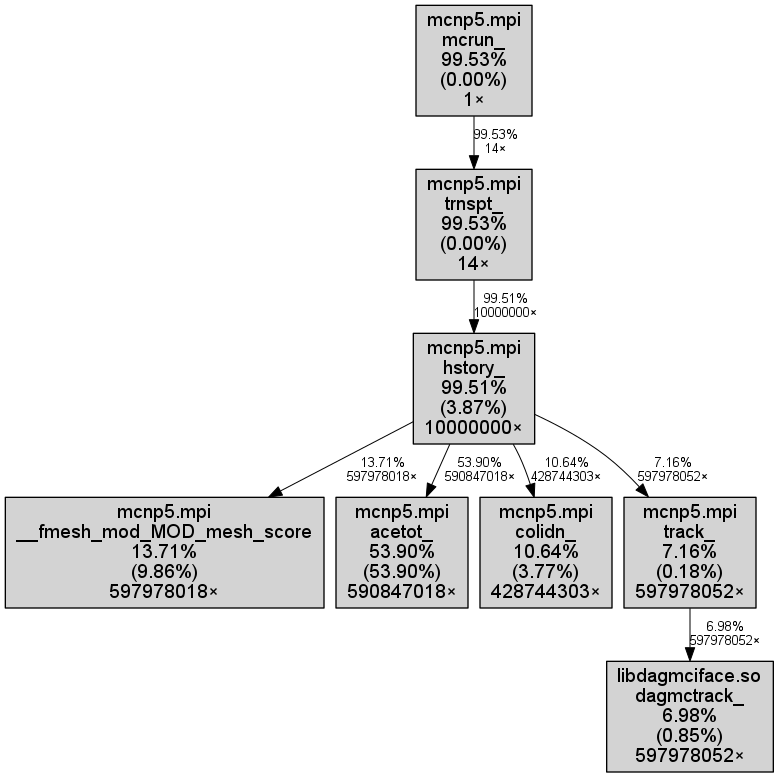
\includegraphics[scale=0.45]{emdag_fng_cg_fine6.png}
  \caption{Call-graph of the EmDAG run on the FNG model for 1E7
    histories. (Processes taking $<=$6\% of the runtime are filtered in order to
    simplify the call-graph.}
  \label{emdag-fng-coarse}  
\end{figure}

While the performance of EmDAG surpasses that of DAGMC, it does not come
as close to the performance of native MCNP as it did in the more simple
transport test models. Upon visually inspecting the faceted FNG model, it was
seen to contain many high valence regions. As an artifact of the variance
reduction used in the intended analysis of this model, many planes were inserted
in the model in order to break up large cells with highly varying particle
intensities. Where these planes intersect the cylindrical volumes of the model,
many high valence regions result as can be seen in Figure
\ref{fng-faceted-models}. As a result it became a curiosity as to whether or
not the high valence regions were being handled better by EmDAG than they were
by DAGMC. In order to test this, the same programs used to do the high valence
vertex study were built using EmDAG and the parameter study of the relative high
valence area and valency was performed. The results in Section \ref{sec:emdag_hv_study}
show that EmDAG also struggles with these high valence regions. In the worst
scenario there is a degradation by two orders of magnitude compared to the best
case scenario which is similar to what seen in the unmodified MOAB ray
tracer. Additionally, it shows degraded performance in the same way that DAGMC
was initially expected to falter - with increasing high valence area and
valency. This is likely due to the nature of the heuristics used by Embree to
construct its acceleration data structures.  Unlike MOAB, however, the BVH
building parameters are not as openly available via Embree's interface.There is,
however, an option to reduce the size of the high valence regions in the mode
within the faceting algorithm by defining a length tolerance.

\begin{figure}[H]
  \small
  \begin{center}
    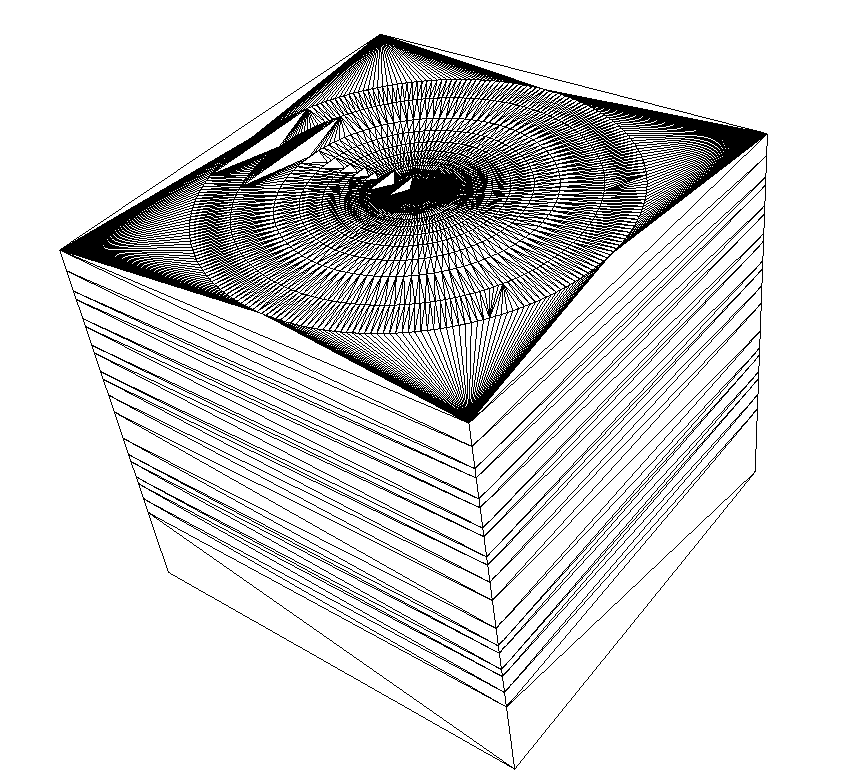
\includegraphics[scale=0.3, trim = 200 0 100 0]{fng_facet_tol.png}
    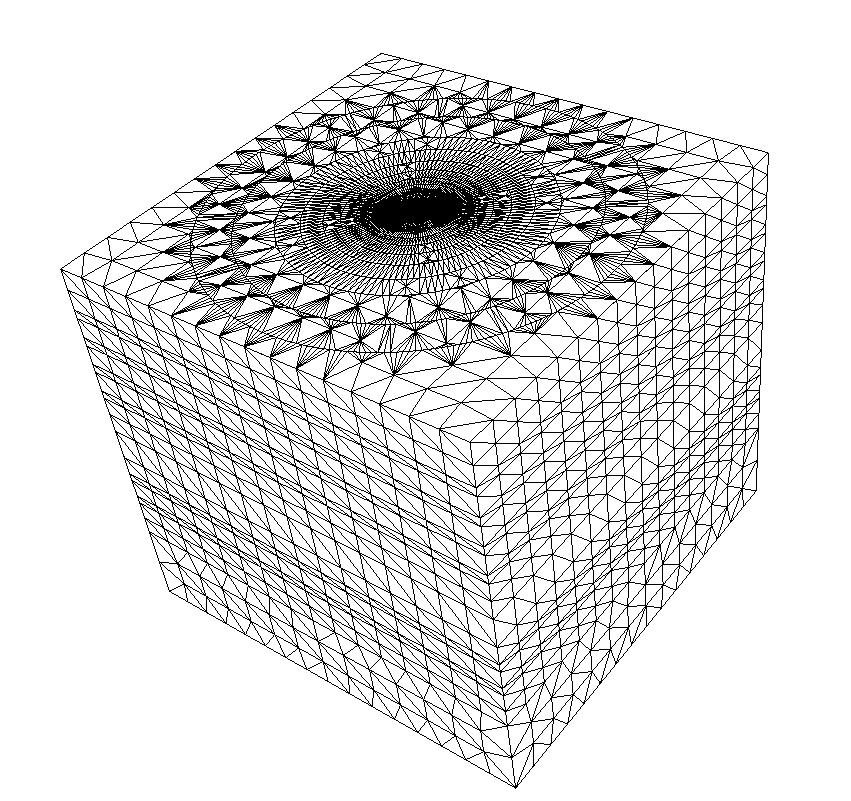
\includegraphics[scale=0.25]{fng_len_tol.png}
    \caption{The FNG faceted model without (left) and with (right) the length
      tolerance applied.}
    \label{fng-faceted-models}
  \end{center}
\end{figure}

The length tolerance is a maximum length for any facet edge returned by the CAD
engine's faceting algorithm. Providing this value to the preprocessing tool
comes at the cost of many more triangles than when supplying only a faceting
tolerance. The difference in facet structure between these models can be seen in
Figure \ref{fng-faceted-models}.

By generating a faceted model using the combination of the length and faceting
tolerances it was hoped that there would be a marked increase in performance
using the EmDAG system and the performance did indeed improve by ~15\%. Due to
the increased number of overall triangles on these planar surfaces, there may be
competing forces at play. As the length tolerance is reduced, the high valence
areas will also be reduced, but the overall number of triangles will increase -
resulting in inherently deeper BVH and longer traversals. Conversely, as the
length tolerance is increased, the number of high valence region areas are
increase, but the number of redundant triangles is reduced improving the average
BVH traversal time enough compensate for a few more rays entering high valence
regions. This observation leads to the idea that length tolerance of the FNG
model could then be optimized. This optimization study, while interesting, will
vary model to model and the results will be complex in nature, depending on the
underlying geometry and geometry adjacent to those regions, etc. In light of the
high valence study results showing that BVH building parameters can be altered
to improve performance and accommodate these high valence regions, it seems that
a better solution is to follow that path over alteration of the mesh globally in
the model. 

\subsection{Limitations}\label{sec:emdag_limitations}

While the implementation of Embree in DAGMC showed a vast improvement in
performance relative to DAGMC's current implementation, several problems were
encountered during the process. This is not surprising when re-purposing a ray
tracing kernel for an unintended application.

One of these problems is the presence of lost particles in a watertight
model. The FNG model EmDAG was tested on is a fully sealed model via the
make\_watertight algorithm. A fully sealed model is one in which every volume is
topologically sealed such that there are no gaps between surfaces or adjacent
volumes. As a result, DAGMC is able to robustly track particles through such a
model with no lost particles. While the lost particle rate for the EmDAG FNG
test relatively low, they in theory should not occur at all as was shown by the
DAGMC runs. After a considerable amount of investigation as to the nature of
these lost particles, their cause was determined to be systematic problem not
encountered in the nested volume cases due to the simple nature of their
geometric topology.

In the DAGMC workflow, a required step for a watertight model is to imprint and
merge the surfaces in the geometry representation before faceting the
model. Imprinting is the process by which surfaces and curves that are
coincident by proximity in space are made the same. This process is accomplished
by splitting entities into their coincident and non-coincident parts. The
merging process then topologically combines these coincident parts into single
entities such that the single entities are topologically adjacent to all
entities bounding the original set of entities that were merged into one. The
result of these steps is non-manifold model with surfaces shared between
neighboring volumes \cite{Smith_2011}.

This imprinting and merging of surfaces allows only one representation of each
topological entity to be created upon faceting the model. By using the faceted
curves of the model as a reference for where surfaces meet in space, the
triangles of a surface are then forced to meet at those curves in a
topologically watertight manner via the \textit{make\_watertight} algorithm
\cite{Smith_2011}. Topologically watertight in reference to triangle facets
refers to shared connectivity of mesh elements between surfaces. This is
distinctly different than watertight by proximity or by points of triangles
being ``close enough'' to one another. Topological watertightness of triangles
refers to the fact that surfaces meshes share connectivity at their
interface. These triangles reference then share mesh vertices in MOAB whose
coordinates in virtual space are represented using the exact same floating point
representation in the database.  In this way particles are cannot be lost
through gaps in surfaces and firing a ray from any position inside a volume
should always result in a triangle intersection. Despite the topological
watertightness of the triangle meshes used in EmDAG, particles were lost in the
transport process.

\begin{figure}[H]
  \centering
  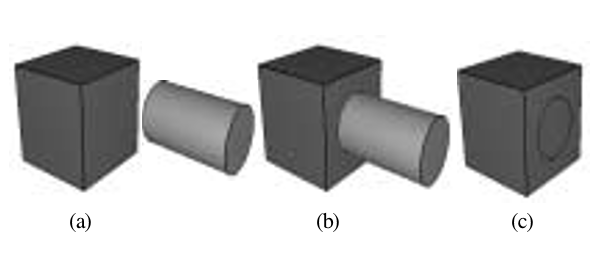
\includegraphics[scale=0.5]{imprint_ex.png}
  \caption{Example of two adjacent volumes being imprinted and merged. a) Two
    volumes, a cube and cylinder are created. b) The cylinder end face is moved
    such that it is coincident with one of the faces of the cube. c) The imprint
    operation is performed and the cylinder curve is imprinted onto the cube
    (cylinder was removed for visibility of imprinted curve). Adapted from
    \cite{White_2002}.}
  \label{imprint_ex}
\end{figure}

Some detailed debugging of this problem revealed that this occurs in a
systematic fashion within the FNG model at intersections of 3 or more
volumes. The scenario is that a particle moves into the intersection between two
surfaces. When this occurs, an intersection with either surface connected to
that interface is a valid hit as the surface is part of the volume the
particle is current positioned within. The particle will then logically move
into the volume on the other side of the hit surface. EmDAG handles most of
these cases well but for the case in which a particle will have a zero track
length inside one of the volumes. A zero track length in this case meaning that
the particles trajectory is such that it will only glance a volume without
having any appreciable track length inside of it. In this case, the EmDAG system
may be unable to find a hit whereas DAGMC's tracking is robust enough to find
the triangle intersection on this volume and move on.

\begin{figure}[h!]
  \begin{centering}
    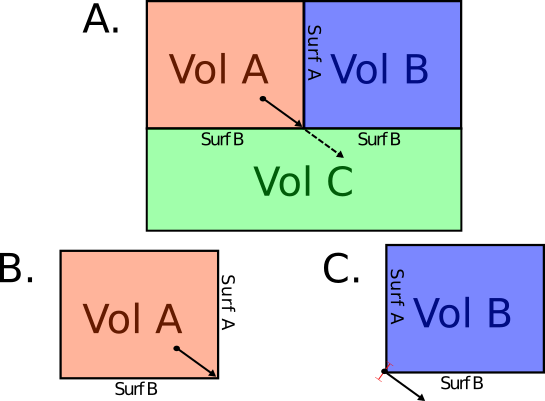
\includegraphics[scale=0.7]{emdag_lost.png}
    \caption{\textbf{A)} The initial scenario of the lost particle. The
      particle's trajectory is such that it intersects with the boundary between
      surfaces A and B. The correct continuation of the particle into volume C
      is depicted as a dashed line. \textbf{B)} An intersection with surface A
      is found though either surface A or B are equally valid. The particles
      position is then updated to its intersection with the boundary of surfaces
      A and B. The particle then logically moves into volume B. \textbf{C)} Upon
      establishment of the particle in volume B the Monte Carlo code requests
      the distance to next surface intersection. The particles position and
      direction are converted from double to single precision. The small change
      in the particle's position places it outside of volume B and the
      trajectory is such that an intersection is not found. At this point the
      particle is considered lost.}
    \label{emdag-lost-particles}
  \end{centering}
  \end{figure}

By isolating this particle's history and producing the particle history with
locations precise enough to detect the discrepancies between EmDAG and DAGMC, it
was found that the position of the particle in EmDAG was numerically too far
outside of a volume to produce the correct triangle hit in either EmDAG or
DAGMC's ray fire systems. The cause of this discrepancy is believed to have to
do with the necessary conversion between double and single floating point
precision in the EmDAG system.

As mentioned before, EmDAG uses single floating point representation in its ray
tracing kernel while DAGMC uses a double precision representation of the
geometry and particle information as does MCNP. In order to accommodate Embree's
representation, properties of the particle location and direction are converted
to single precision for ray tracing queries in Embree and back to double
precision when in DAGMC. When changing the floating point representation,
rounding rules based on the computing environment are used to determine the new
representation according to IEEE standards for conversion between precision
levels \cite{IEEE_STD_2008}. These changes in the particle's location and
direction are small, but in the scenario described above it seems that the
particle location and/or direction are altered enough throughout the course of
its history to cause a failed ray intersection - resulting in a lost particle.

In Brandon Smith's thesis, ``Robust Particle Tracking and Advanced Geometry for
Monte Carlo Radiation Transport'' \cite{Smith_2011} there is a detailed
description of the different pathologies encountered in tracking particles
through a surface mesh representation of a geometric model. Briefly mentioned in
this chapter is the possibility of a lost particle due to numerical error in the
particle's position perpendicular to the particle's trajectory. Lost particles
caused by this pathology are not covered however as the double floating point
representation does not allow the particle position to change enough for this
case to occur in practice. In EmDAG, however, this particular pathology is now
vulnerable due to the constant conversion from single to double precision values
between DAGMC and Embree. In order to avoid this problem moving forward, any
improvements to DAGMC's ray tracing kernel for particle tracking will need to
maintain use of double precision representations for mesh elements for robust
coupling of numerical and logical particle positions and directions.

\section{A Mixed Precision BVH}

As described in Section \ref{sec:emdag_limitations} a SIMD-oriented ray tracing
kernel was successfully implemented and applied in DAGMC. Unfortunately, this
system was inherently limited by conversion from single to double precision
values. The use of double precision intersections is required for DAGMC to
successfully interface with any of the Monte Carlo it supports. As a result,
reduction of the triangle primitives to single precision is not an option.

This section outlines an approach to using single precision bounding volumes
around double precision geometric primitives. Because the majority of the
computational work in ray tracing occurs in traversing the BVH as opposed to
testing triangles for intersection, it is hypothesized that the majority of the
performance benefits seen in the EmDAG implementation can be preserved in the
proposed mixed precision system, dubbed the Mixed Precision Bounding Volume
Hierarchy (MPBVH).

\subsection{Implementation and Design}

The MPBVH was created by the author as an independent project which draws on
design elements from Embree while interfacing with MOAB to optimize CPU-based
ray tracing for the application of CAD-based Monte Carlo Radiation
Transport. Several such design elements found in both the Embree and the MPBVH
include:

\begin{itemize}
  \item single-precision bounding entities
  \item bit-encoding of node types
  \item type-agnostic vectors to support SIMD instruction sets
  \item memory pre-fetching of node memory added to the traversal stack
  \item pre-computation of near and far box boundaries
  \item vectorized node intersection
\end{itemize}

The details of these features can be found in Embree's GitHub repository
\cite{Embree}. Embree supports many geometric types such as 

The kernel created by the author is a lightweight version of the
Embree kernel focused on static triangle meshses and access to an external mesh
database used for engineering analysis. This allowed for several improvements in
both robustness and memory usage in comparison to the EmDAG system. The
remainder of this section will address some of these features and design
changes.

\subsubsection{MOAB Direct Access}

MOAB provides a rich interface used to create, modify, and query both structured
and unstructured mesh representations. It supports many meta-data types as well as
the arbitrary grouping of mesh entities into sets to represent boundary
conditions, material types, etc. MOAB also allows direct access to memory which
is normally protected through its standard interface. This allows for rapid look
ups data and allows other applications access to the memory as well. This
capability can be extremely useful in data transfer or query based operations,
such as ray tracing.

The MPBVH uses these methods to populate references to triangles in
the BVH without needing to duplicate their coordinate values or
connectivity. Access to these locations in memory is handled by a direct access
manager object which protects the mesh information from modification during the
building and traversal of the BVH. All coordinate and connectivity information
accessed through this manager, which protects against modification of MOAB's
memory.

Information is looked up via offset values using handles for triangle and vertex
entities. This allows coordinates values for triangle intersections to be
gathered optimally from the database. Bypassing the MOAB interface in this way
requires that there are no gaps or ``holes'' in the set of handles representing
entities, that the set of entity handles in the database is contiguous.

Fortunately, files loaded into MOAB have a contiguous entity handle space
regardless of the contiguity at the time the file was written to disk. This
guarantees that the set of entity handles representing DAGMC geometries will be
contiguous when loading a geometry for simulation. If the mesh data is modified,
in particular if entities are deleted, then this requirement will be broken and
it may not be possible to use the direct access methods robustly. DAGMC does not
modify mesh data once the file has been loaded for simulation. MOAB provides
tools for collapsing or modifying the entity handle space if this becomes
necessary in future applications of DAGMC.

\subsubsection{Reduced-Precision Ray Tracing}\label{subsubsec:reduced_precision}

In the SIMD BVH kernel, bounding boxes are calculated in single precision based
on double precision triangle coordinates from the MOAB direct access manager. As
demonstrated by the limitations of the EmDAG implementation, double precision
intersections with triangle primitives are necessary for robust radiation
transport in CAD geometries.

Using double precision ray values to intersect with single precision boxes is
possible due to IEEE standards used to truncate double precision values to single
precision values, but costly due to the conversion of the ray origin and
direction for each box intersection \cite{IEEE_STD_2008}. Instead, a method was
applied in which a traversal ray data structure is used represent the ray origin
and direction in single precision. This greatly accelerates the traversal
process moving through the hierarchy of bounding boxes. Once leaf nodes are
reached in the tree, the original double precision values of the ray and double
precision triangle coordinates are used to calculate intersections and return
distances to the surface.

\begin{figure}[H]
  \centering
  \includesvg{../images/reduced_precision_scheme}{0.6\textwidth}
  \caption{The reduced precision scheme used to accelerate ray traversal while
    returning double precision intersections.}
  \label{fig:reduced_precision_scheme}
\end{figure}

This method removes the need for conversion of single precision intersection
distances which caused lost particles in the EmDAG implementation, but there are
other robustness concerns which must be addressed. In order to return the
correct intersection distance, the leaf node containing the triangle which
intersects with the ray at that distance must be visited. Upon converting ray
origins and directions from double to single precision, small changes in the ray
origin and direction are introduced. This effect is illustrated in Figure
\ref{fig:double_to_single_ray}.

\begin{figure}[H]
  \centering
  \includesvg{../images/double_ray_float_ray}{0.5\textwidth}
  \caption{A representation of the directional change due to conversion of a
    ray's origin and direction from double to single precision. Where capital
    letters indicate double precision values.}
  \label{fig:double_to_single_ray}
\end{figure}

To ensure that node visits which would occur in double precision will also occur
in single precision, the bounding boxes are artificially enlarged by a small
amount to ensure that this is true. When determining how much the boxes need to
be enlarged, it is important to understand the difference in the intersection
locations caused by this change.

Let the original, double precision, ray be $\vec{R}$ where its direction is

$$ \vec{D} = < R_{u}, R_{v}, R_{w} > $$

and the traversal ray, in single precision, be $\vec{r}$ where its direction is

$$ \vec{d} = < r_{u}, r_{v}, r_{w} > $$

Where the distance between these two vectors at their unit length
can be described as.

$$ \Delta = \sqrt{ (R_{u} - r_{u})^{2} + (R_{v} - r_{v})^{2} + (R_{w} -
  r_{w})^{2} } $$

Because the difference between the vectors in each dimension is representative
of the truncation of double precision values to single precision, they can be
set equal to a value $\delta$.

$$ \delta = R_{u} - r_{u} = R_{v} - r_{v} = R_{w} -  r_{w} $$

By substituting this value, $\Delta$ becomes

$$ \Delta = \sqrt{3} \delta $$

Extending this to a ray traveling a parametric distance, $t$, along the
respective single and double precision ray directions, the value of $\Delta$
becomes

$$ \Delta = \sqrt{ (tR_{u} - tr_{u})^{2} + (tR_{v} - tr_{v})^{2} + (tR_{w} -
  tr_{w})^{2} } $$

$$ \Delta = \sqrt{3} t \delta $$

This equation indicates that boxes will need to be expanded an amount $\Delta$
in order to ensure that $\vec{r}$ will intersect any box $\vec{R}$ does. One
concern with this expansion is that artificially extending the bounding boxes
causes more overlap and raises the average number of nodes visited per traversal
of the BVH. If the value of $\Delta$ is a large value, then the performance of
tracing rays through the data structure may suffer. An examination of the
$\Delta$ value indicates that this is not the case, however.

As a worst-case consideration, $t$ should be evaluated as the maximum distance a
particle might travel through the geometry. This can be evaluated as the longest
possible diagonal of the problem's global bounding box using it's largest
dimension, $l_{max}$.

$$ t_{max} = \sqrt{3} l_{max} $$

Given this value, the truncation will be, in the worst case, $10^{7}$ on modern
CPU systems. This value can be considered to be relative to the overall
geometric scale of the problem, represented by $t_{max}$. Using this analysis,
the value of $\Delta_{max}$ can be written as 

\begin{equation}
  \centering
  \Delta_{max} = 3 x 10^{-7} l_{max}
  \label{eq:box_extension_limit}
\end{equation}

Another method for working with mixed precision BVHs in double precision
geometries was put forth by Vaidyanathan in which the ray's origin is
periodically updated during traversal so that the deviation from the double
precision intersection is limited \cite{Vaidyanathan_2016}. This method is
intended for use with geometries in motion and requires additional computation
during ray traversal. DAGMC geometries, and Monte Carlo radiation transport
geometries in general, are static, so it is more efficient to account for the
discrepancy caused by the reduced precision ray direction during construction of
the MPBVH.

To further understand this effect, the value of the box extension in the kernel
was varied from \num{1E-8} to \num{1E2}. For each box extension value, the same
set of ray fire tests in Section \ref{subsubsec:emdag_rf_performance} were
run. The average of the ray fire times over all faceting tolerances is used as a
representative value in Figure \ref{fig:box_bump_tests} to described the
performance for each model. Performance of the MPBVH kernel isn't strongly
effected below $\Delta$ values of \num{1E-2}. Above this value, the performance
degrades rapidly as box overlaps become large and the false positive
intersections of the ray with nodes in the tree dominates the run time. When the
extension of the boxes becomes large enough, the runtimes plateau - indicating
that every node in the tree is being visited for each ray fire. Below a value of
\num{1e-6}, missed rays begin to appear in the runs. The threshold for this
region can be predicted using the model in Equation
\ref{eq:box_extension_limit}. The longest dimension for any of the models ranges
from 10 to 50 units in size. Inserting this into Equation
\ref{eq:box_extension_limit} indicates that missed rays will start occur at
values of $\Delta$ = ~\num{3E-6}. These boundaries leave a significant room for
box extension values which do not affect performance or robustness of the
kernel.

\begin{figure}[H]
  \centering
  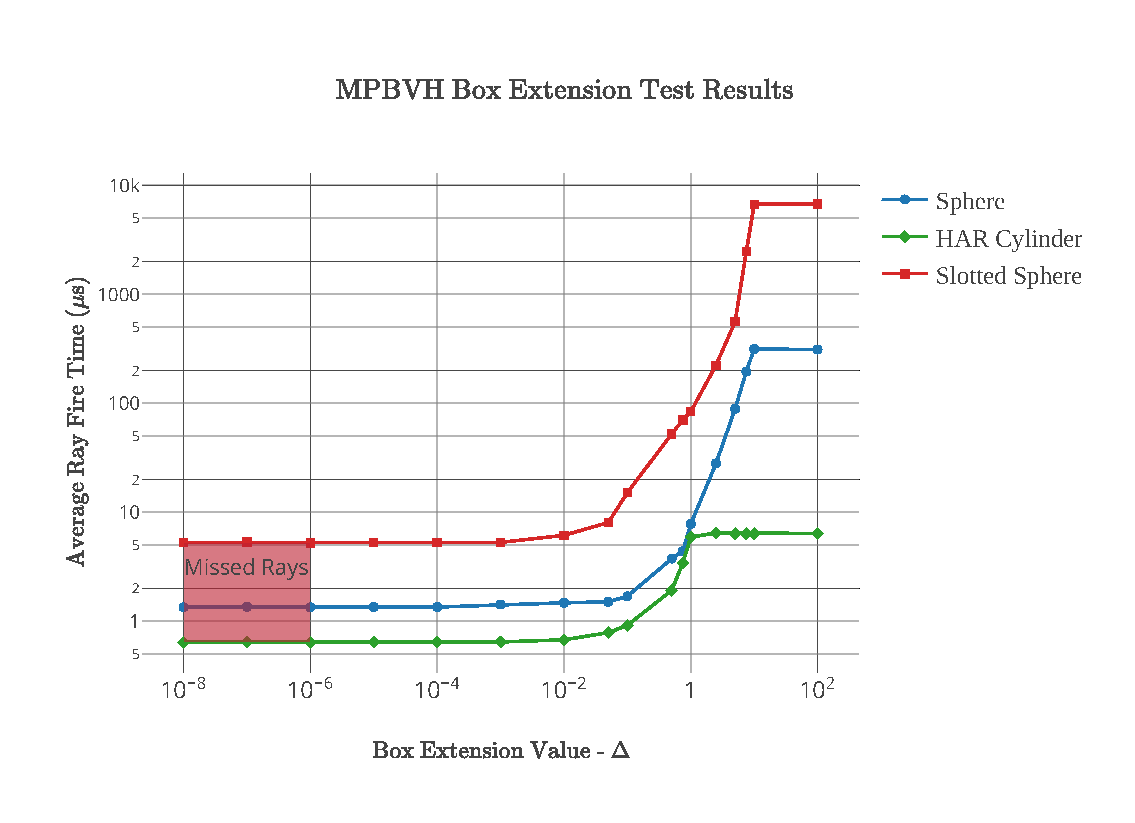
\includegraphics[scale=0.8]{box_extension_test.eps}
%  \includesvg{../images/box_extension_test}{0.8\textwidth}
  \caption{Study of ray tracing performance and robustness for various values of
    the box extension parameter, $\Delta$. 600,000 rays were fired at each model
    for faceting tolerance values ranging from. Points in the graph represent
    the average over all faceting tolerances used.}
  \label{fig:box_bump_tests}
\end{figure}

The biggest geometric problem examined in this work is the ITER-BLITE model. The
largest side of the global bounding box in this model is $4 \, \text{x} \,
10^{3}$ cm. Using this as a representative value of $l_{max}$ results in a box
expansion value, $\Delta$, of $1.2 \, \text{x} \, 10^{-3}$. This value is small
enough to cause minimal overlap in the bounding boxes and a negligible effect on
the BVH performance, as seen in Figure \ref{fig:box_bump_tests}. For all results
discussed in this work $\Delta$ was set to $5 \, \text{x} \, 10 ^{-3}$.

\subsubsection{Simplified Surface Area Heuristic}

The MPBVH employs a modified version of the Surface Area Heuristic,
discussed in Chapter \ref{ch:background}, which was developed by the
author. This version of the heuristic, dubbed the Simplified Surface Area
Heuristic (SSAH), removes estimation of the relative cost between a tree
traversal step and a primitive intersection.

This version of the heuristic considers the cost of traversal, $C_{t}$, to be
small compared to the cost of a triangle primitive intersection, $C_{i}$. This
assumption is stronger due to the mixed precision nature of the implementation
than for systems in which the hierarchy and primitives are both stored with the
same precision.

After these considerations, the cost evaluation for a candidate node can be
evaluated as seen in Equation \ref{eq:simplified_sah}.

\begin{figure}[H]
  \begin{align}
&C =  \cancel{C_{t} +} \frac{SA_{L}}{SA_{P}} |P_{L}|C_{i} + \frac{SA_{R}}{SA_{P}} |P_{R}|C_{i} \\
&C_{g} = \frac{SA_{L}}{SA_{P}} |P_{L}| +  \frac{SA_{R}}{SA_{P}}|P_{R}| \\
&C = C_{i}C_{g}
  \end{align}
  \begin{align*}
    C^{L} = C_{i} C^{L}_{g} \\
    C^{R} = C_{i} C^{R}_{g} \\
    C^{L} < C^{R} \\
    C_{i}C^{L}_{g} < C_{i}C^{R}_{g}
  \end{align*}
  \begin{align}
    C_{simplified} = C_{g} = \frac{SA_{L}}{SA_{P}} |P_{L}| +
    \frac{SA_{R}}{SA_{P}}|P_{R}|
    \label{eq:simplified_sah}
  \end{align}

  \begin{align*}
    C_{t} - & \,cost\, of\, traversal\, to\, child\, nodes \\
    C_{i} - & \, cost\, of\, primitive\, intersection\, check\, \\
    SA_{L} - &  \,surface\, area\, of\, left\, child \\
    P_{L} - & \, primitives\, contained\, by\, the\, left\, child  \\
    SA_{R} - & \, surface\, area\, of\, right\, child \\
    P_{R} - & \, primitives\, contained\, by\, the\, right\, child \\
    SA_{P} - & \, parent\, bounding\, volume \\
    C^{L} \text{,} C^{R} - & \, left \, and \, right \, child \, costs, \, respectively, \, in \, a \, binary \, tree
  \end{align*}
  
  \caption{A form of the simplified surface area heuristic for a binary tree.}
  \label{fig:SSAH}
\end{figure}

By neglecting the traversal cost, the cost of the node can be broken into two
components, the cost of the intersection, $C_{i}$ and the geometric cost,
$C_{g}$. Because these values are used in a purely relative manner to compare
the costs of candidate splits, the constant factor of the primitive intersection
is no longer required. This form of the heuristic is purely a weighted geometric
evaluation without estimation of implementation-based valued which can vary
based on machine architecture, build settings, etc.

\subsubsection{Surface Root Nodes}

In DAGMC, trees are created for each volume and surface in the geometry. Rather
than duplicate surface trees for each volume they appear in, one tree is created
for each surface and for each volume the resepective surface trees are joined
into a single tree. This avoids duplication of tree information and minimizes
the memory footprint of DAGMC. It is critical to DAGMC that the surface
intersected is returned as part of the ray's intersection information so that
particles can be passed from volume to volume correctly. This information is
maintained in the root nodes of surface trees and updated during the BVH
traversal process. In order to maintain this functionality without duplicating
triangle information, a similar scheme was implemented in the MPBVH, but within
the framework of a BVH design for SIMD traversals.

Tree nodes in both Embree and the MPBVH are represented by a node
reference construct which stores a single pointer value as an integer
representation. All stored constructs, namely the bounding nodes and primitive
references, in the BVH are designed to be 16-byte aligned in memory, leaving the
4 least significant bits of the integer-stored pointer value unused. These bits
are used to encode information about leaf nodes in the tree. When the true
pointer to either an interior node or leaf node is needed, the pointer value is
recovered by setting these bits to zero and casting the pointer to the
appropriate object type.

\begin{figure}[H]
  \centering
  \includesvg{../images/quad_tree_sets}{0.8\textwidth}
  \caption{A representation of how surface BVHs are joined into a volume BVH.}
  \label{fig:quad_tree_sets}
\end{figure}

In a leaf node reference the fourth bit is set to one, indicating it is a leaf
node and that any pointer value taken from the node reference should be treated
as a pointer to a primitive reference. The remaining three bits in the integer are
combined to indicate the number of primitives in that leaf node. This places a
limit of eight on the number of entities stored in a leaf node. The impact of
this limit will be discussed further in Chapter \ref{ch:high_valence}.

\begin{figure}[H]
  \centering
  \includesvg{../images/leaf_encoding}{1.0\textwidth}
  \caption{Visual representation of leaf encoding using integer-based
    pointer values in node references.}
  \label{fig:leaf_encoding}
\end{figure}

In DAGMC, a BVH is created for each set of triangles representing a
surface. These surface trees are then joined into a single tree that represents
a volume as depicted in Figure \ref{fig:quad_tree_sets}. This avoids duplication
of surface trees for each volume. It also allows the return of which surface is
intersected, allowing for optimized transport of a particle to the volume on the
other side of that surface via the topology represented by the mesh hierarchy
described in Section \ref{sec:emdag_transfer}. Embree allows for a similar model
in which surfaces are represented as ``geometries'' rather than surfaces. Those
geometries can be grouped into ``scenes'' rather than surfaces.  The creation of
a special node to represent the root of a surface tree was implemented to
provide this information. This node type is an extended node reference which
contains additional information about the surface the tree is constructed
around. In particular, this node stores the id of the surface and its sense
information relative to the volumes on either side of the surface. This sense
information is used to automatically adjust the returned triangle normals for
any intersections with that surface, and avoids the duplication of triangle
connectivity that was necessary in the EmDAG implementation.

The set leaf node reference is identified by toggling the least significant bit in
the reference's integer value. Because only the first bit is altered, this node
is not recognized as a leaf containing primitives but rather a leaf of the
volume tree. Information about the current surface being visited and the sense
information is updated on the traversal ray and used to set any hit information
on the returned ray. The pointer value stored by the node reference is a pointer
to the node reference for the bounding element at the top of the
surface tree. This node is pushed onto the stack and the traversal continues
uninterrupted.

The depth-first traversal of the hierarchy protects against
any invalid surface information being set on the ray as the all nodes underneath
that surface will be visited before moving on to the next surface, at which
point the traversal ray information will be updated.

\begin{figure}
  \includesvg{../images/set_leaf_encoding}{1.0\textwidth}
  \caption{Visual representation of set leaf encoding using integer-based
    pointer values.}
  \label{fig:set_leaf_encoding}
\end{figure}

This node type also provides the ability to avoid duplication of triangle
connectivity to represent sense-adjusted triangle normals as was required in the
EmDAG system to track the relative surface-to-volume senses. A MOAB lookup of
this sense information after returning ray hits is also a viable option, but it
would be relatively expensive to in comparison to adjusting triangle normals on
the fly.

\subsection{Robustness Testing}

The the criterion for a robust ray tracing kernel are as follows:

\begin{itemize}
  \item every ray query should return the \textbf{same triangle id} as MOAB's BVH
    implementation
  \item every ray query should return the \textbf{same intersection distance} as MOAB's BVH
\end{itemize}

To meet these criterion the Pl\"{u}cker ray-triangle intersection test used in
MOAB is also used in the MPBVH \cite{Platis_2003}. Many unit tests are used to
ensure watertight box intersection using the slab method \cite{Kay_1986} in
single precision, but the mixed precision scheme is best tested using DAGMC
models. In MOAB, the Pl\"{u}cker ray triangle intersection method is used to provide
watertight intersections with triangle meshses \cite{Platis_2003}. The same
algorithm was applied in the MPBVH to ensure that simulation results using both
the MPBVH and MOAB BVH are consistent. Several unit tests in the kernel fire
rays from the center of single-volume DAGMC models with rays directed at
the vertices, edges, and center of each triangle in the model. These tests
ensure that the same triangle is hit and \textit{exactly} the same intersection
distance is returned in either system.

Missed rays and lost particles are also monitored in testing the ray fire
performance and in particle transport, though none were found outside of the
controlled box extension study in Section \ref{subsubsec:reduced_precision}.

\subsection{Ray Fire Performance}\label{sec:mpbvh_rf_perf}

The same set of ray fire performance tests were run as in Section
\ref{subsubsec:emdag_rf_performance}. As shown in Figure
\ref{fig:mpbvh_rf_tests}, the MPBVH shows a significant improvement compared to
the current implementation in MOAB and comparable to the EmDAG implementation.

\begin{figure}[H]
  \centering
  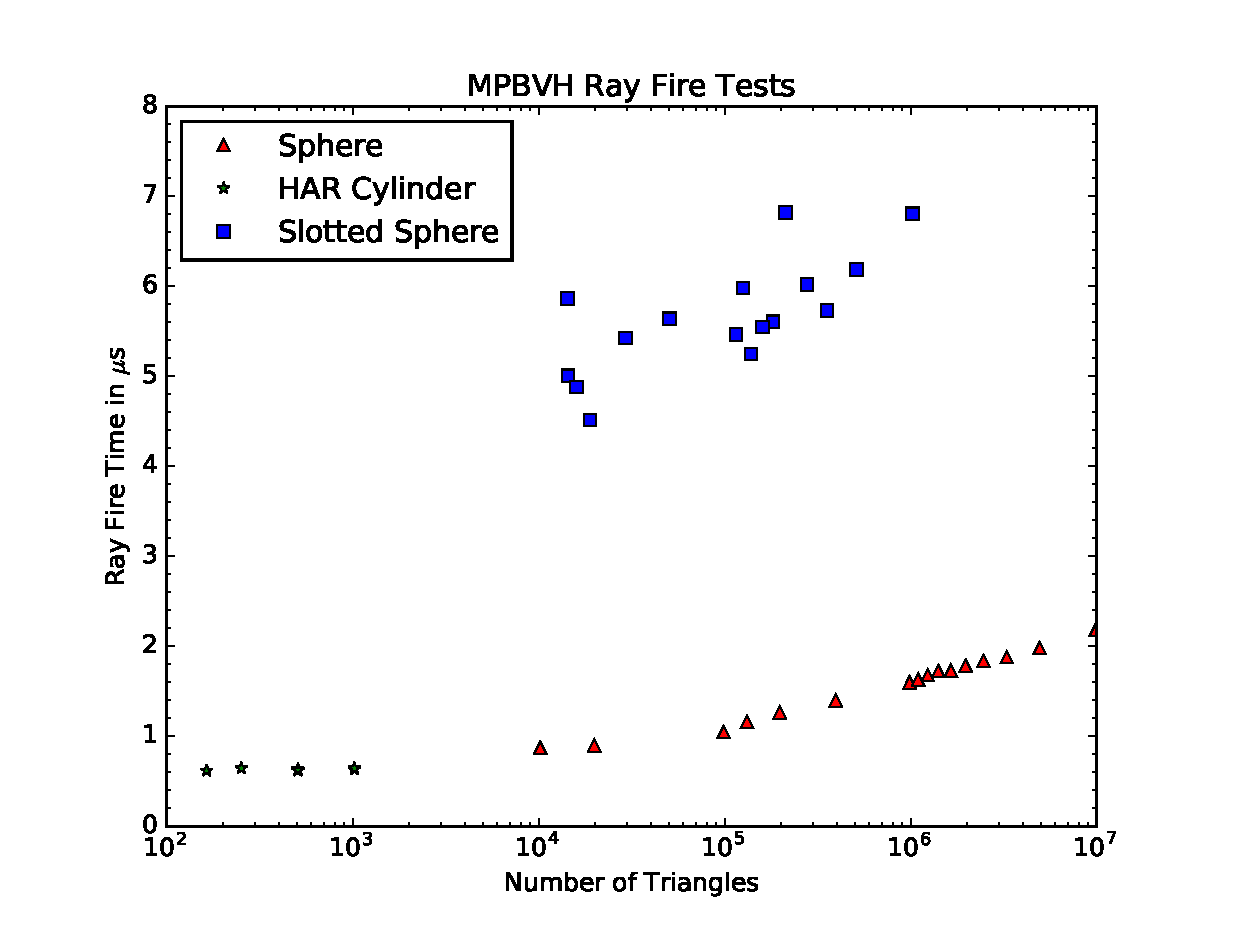
\includegraphics[scale=0.33]{mpbvh_rf.eps}
  \caption{Average ray fire times for the MPBVH for a sphere, slotted sphere, and High Aspect Ratio (HAR) cylinder.}
  \label{fig:mpbvh_rf_tests}
\end{figure}

\section{Simplified Particle Tracking}

The MPBVH kernel has been implemented in DAGMC as a numerically based particle
tracking tool using a simple algorithm for determining \textit{Next Surface}
queries and \textit{Point Containment} queries. Previously, additional logical
work was used to avoid lost particles and infinite loops in particle
histories. This tracking algorithm uses structures known as the \textbf{MBRay}
(short for MOAB Ray) and \textbf{MBAccumulatorRay}. Both of these structures
(shown in Figure \ref{fig:mpbvh_ray_structures}) are critical to the use of the
MPBVH as a robust particle tracking tool.

\begin{lstlisting}[language=Python,basicstyle=\tiny]
  def next_surface(current_volume,
                   point,
                   direction,
                   dist_limit
                   &next_surface,
                   &next_surface_distance):

      # create a ray with infinite length
      ray = MBRay(point,direction)
      ray.volID = current_volume
    
      # if the ray orientation is set, ignore
      # hits which opposed the triangle's
      # sense-adjusted normal
      if ray_orientation == 1 :
        set_filter(backface_cull)
      # if the orientation is not set, remove the filter
      else:
        unset_filter()
    
      # fire the ray
      fire_ray(ray)
    
      # if the ray missed and overlaps are allowed in the model
      # fire a ray in the opposite direction
      if ray.surfID == -1 and get_overlap_thickness() != 0.0: {
        small_val = get_overlap_thickness() * 0.01
        ray.direction *= -1
        # apply some small space at the beginning of the ray
        # where hits are ignored
        ray.tnear = small_val
        # set the ray distance to the overlap thickness
        ray.tfar = get_overlap_thickness()
    
        # unset the ray filter regardless of the ray orientation
        unset_filter()
    
        fire_ray(ray)
        
        # update ray value to zero for this type of hit
        ray.tfar = 0
    
      # if we have a hit at this point, set the returned
      # surface ID and distance
      if ray.surfID != -1:
        next_surf = ray.surfID
        next_surf_distance = ray.tfar

      # otherwise the particle is lost,
      # set return information accordingly
      else:
        next_surf = 0
        next_surf_distance = ray.tfar
    
        return

  def backface_cull( &mbray ):

      # if the ray direction opposes the hit triangle's
      # normal vector, reject the ray hit
      if dot_product(mbray.dir, mbray.norm) < 0.0:
          mbray.geomID = -1
          mbray.primID = -1

      return

      \caption{The method used for \textit{Next Surface} queries.}
      \label{alg:Next Surface Pseudo Code}
\end{lstlisting}

The algorithm in Figure \ref{alg:Next Surface Pseudo Code} avoids many logical
checks and the classification of hit locations for repeated hits. It also avoids
mesh database lookups of adjacent triangles for edge and node hits. This used to
be necessary due to the ray history passed into the \textit{Next Surface} query,
causing rays to sometimes become stuck in what was referred to as the
``pinwheel'' loop. The ray history was as an optimization to avoid repeated
intersections with the same triangle. By abandoning this construct and relying
entirely on the performance of the underlying ray tracing kernel, the algorithm
can be simplified to always return the nearest intersection. Infinite loops in
which particles oscillate between volumes on a surface boundary are addressed by
returning exiting intersections only.

\begin{figure}[H]
  \centering
  \includesvg{../images/mbray_structs}{1.0\textwidth}
  \caption{Ray structures used to communicate hit information between the MPBVH and DAGMC.}
  \label{fig:mpbvh_ray_structures}  
\end{figure}

The conditions laid out for a robust tracking
algorithm by B. Smith are as follows \cite{Smith_2011}:

\begin{enumerate}[a]
  \item Particles cannot become lost
  \item Infinite loops cannot occur
\end{enumerate}

The algorithm presented here addresses \textbf{a)} by using the watertight
Pl\"{u}cker intersection test and extending ray boxes to ensure the correct
triangle is checked for intersection. Part \textbf{b)} is addressed by firing a
ray in the opposite direction if the initial ray does not find an
intersection. The scenario here being that the particle is inside a
self-intersecting or overlapping volume. To avoid a zero-distance hit when
firing in the opposite direction, a small value is also set as the ray's
near-side parameter. In traversal, any hits closer than this value will be
ignored. The ray's length is also set to the allowed overlap thickness. Any
intersections beyond this distance are ignored as well. Thus an exiting
intersection in the overlap region can be found and a zero-distance intersection
will be returned from the \textit{Next Surface} query.

The MPBVH provides the capability to set callback functions used to filter and
validate ray intersections, as demonstrated by the \textit{backface\_cull}
function above. These filter functions can also be used to accumulate ray hits,
which is critical to implementation of a robust point containment algorithm
based on the MPBVH, shown in Figure \ref{alg:Point Containment Pseudo Code}.

\begin{lstlisting}[language=Python,basicstyle=\tiny]
  def point_contained( volume, point, direction, &result):
      # result values : 0 - outside; 1 - inside

      # start with an outside value
      result = 0
  
      # if a direction was not supplied,
      # generate a random one
      if not direction:
          direction = get_random_direction()

      # create a ray
      ray = MBRay(point, direction)
      ray.volID = volume

      # accept ray hits regardless of
      # orientation w.r.t. triangle normal
      unset_filter()

      # fire the ray
      fire_ray(ray)
      # calculate the dot product of
      # ray direction and triangle normal
      dot_prod= dot_product(ray.dir, ray.norm)
      
      # if a hit is found, 
      if ray.geomID != -1 and dot_prod != 0.0:
          if dot_prod < 0.0:
              result = 1
          else:
              result = 0
         return

      # if the ray is tangent, the overlap thickness is
      # non-zero, or it missed - 
      # count hits and sum orientations
      if dot_prod == 0.0 or get_overlap_thickness() > 0.0:
         aray = MBAccumulatorRay aray(point, direction)
         aray.volID = volume

         set_filter(count_hits)

         fire_ray(ray)

         # if no hits were found
         # point is outside
         if aray.num_hit == 0:
             result = 0
             return

         # fire ray in negative direction
         # and reset length
         aray.dir *= -1
         aray.tfar = inf;

         fire_ray(aray)
         
         # if no hits were found
         # point is outside
         if aray.num_hit == 0:
             result = 0
             return
            
         # check the value of the sum
         if 0 > aray.sum:
            result = 1
         else:
            result = 0
            
      return       

  def count_hits( &aray ):
      if dot_product(aray.dir, aray.norm) > 0.0:
          aray.sum -= 1 # exiting hit
      else:
          aray.sum += 1 # entering hit          

      # always reset ray hit values
      aray.geomID = -1
      aray.primID = -1

      # increment number of hits
      aray.num_hit++

      return
      \caption{Algoritm for determining point containment within a volume.}
      \label{alg:Point Containment Pseudo Code}
\end{lstlisting}

In this method the ray is intersected with the volume and a hit is evaluated as
either entering or exiting based on the dot product calculation with the
sense-adjusted triangle normal. If the ray finds no intersection and any of the
following conditions are true:

\begin{itemize}
  \item the ray misses the volume
  \item the ray direction is tangent to the intersected triangle normal
  \item the overlap tolerance is non-zero
\end{itemize}

Then ray hits are accumulated by firing a \textbf{MBAccumulatorRay} in both the
positive and negative direction. All hits are registered on the ray as exiting
or entering based on the dot product calculation of the direction and triangle
normal (see the \textit{count\_hits} function). If no hits are found, then the
point is outside of the volume. If hits are found, the sign of the summation
value indicates whether more exiting or entering hits were found. If more
exiting than entering hits are found, then the particle is considered to be
inside the volume. Otherwise it is considered to be outside of the volume.

This algorithm was applied to all of the simulation results presented in this
chapter without lost particles or causing infinite loops.

\subsection{Simulation Results}

\subsubsection{Simple Test Cases}\label{subsec:mpbvh_simple_tests}
The MPBVH kernel was applied as the ray tracing kernel for the same set of
transport test cases as the EmDAG implementation. Table
\ref{tab:mpbvh_transport_timing_simple} shows the results of tests. The MPBVH
implementation performs comparably to EmDAG for the cube and nested cubes cases,
but is significantly slower in the sphere and nested spheres cases. This is
expected based on the difference in pure ray fire times from Section
\ref{sec:mpbvh_rf_perf}

\begin{table}[H]
  \small
  \begin{center}
    \begin{tabular}{lccc}

      \toprule
      Test Model & MCNP & DAG-MCNP & DAG-MCNP (w/ MPBVH) \\
      %%\hline
      & \multicolumn{3}{c}{\textbf{time (min)/ ratio to MCNP}} \\
      \hline
      Sphere         & 2.93 / 1.00 & 25.13 / 8.58  & 9.38 / 3.2  \\
      Cube           & 5.03 / 1.00 & 10.56 / 2.10 & 5.46 / 1.08 \\
      Nested Spheres & 4.35 / 1.00  & 50.82 / 11.68  & 9.88 / 2.27 \\
      Nested Cubes   & 4.73 / 1.00 & 9.26 / 1.96 & 4.09 / 0.86 \\
      \bottomrule
    \end{tabular}
  \end{center}
  \caption{Runtime comparison native MCNP, DAG-MCNP, and DAG-MCNP using the
    MPBVH over four transport test problems. No lost particles occurred in any of
  these runs and all results match the standard DAGMC implementation exactly.}
  \label{tab:mpbvh_transport_timing_simple}
\end{table}

\subsubsection{Production Simulations}\label{subsec:mpbvh_production_transport}

After verifying that no particles were lost in the simple test cases, the MPBVH
implementation of DAGMC was applied to the same FNG model as EmDAG. The results
of this simulation can be seen in Table
\ref{tab:mpbvh_transport_timing_production}. In contrast to the EmDAG system, no
lost particles were found in the FNG simulation with a volumetric source and all
tally results matched the standard DAGMC implementation with reduction in the
runtime by over a factor of two. Due to the success of the DAGMC MPBVH
implementation for the FNG model, this system was applied to several other
production models as well.

\begin{table}[H]
  \small
  \begin{center}
    \begin{tabular}{lccc}

      \toprule
      Test Model & MCNP & DAG-MCNP & DAG-MCNP MPBVH \\
      %%\hline
      & \multicolumn{3}{c}{\textbf{time (min)/ ratio to MCNP}} \\
      \hline
      FNG           & 2.49 / 1.00 &  9.83  / 3.95  & 6.48 / 2.60 \\
      ATR           & 3.18 / 1.00 &  36.16 / 11.37 & 8.54 / 2.68 \\
      UWNR          & 270  / 1.00 &  7900  / 29.26 & 3645 / 13.5 \\
      ITER-BLITE    & N/A  / 1.00 &  116   / N/A   & 44   / N/A  \\
      \bottomrule
    \end{tabular}
  \end{center}
  \caption{Runtime comparison native MCNP, DAG-MCNP, and DAG-MCNP using the
    MPBVH over four transport test problems. No lost particles occurred in any of
  these runs and all results match the standard DAGMC implementation exactly.}
  \label{tab:mpbvh_transport_timing_production}
\end{table}

\section{Limitations and Future Work}

%\subsection{Closest to Location}

\subsection{Large Models}

As discussed in Section \ref{subsubsec:reduced_precision}, the box extension
value may need to be varied depending on the size of the model. The value
currently applied in the kernel is suitable for the majority of the models used
in DAGMC. The study on this value indicates that it could be increased
significantly to retain robustness in models of a larger geometric scale without
detriment to the performance of the simulation.

In the future, this extension value could be set on a volume-by-volume basis as
intersection distances in DAGMC should never exceed the maximum chord length of
a volume before being considered lost. This would limit the performance
degradation for models of a large global scale with small, local volumes.

Though this work does not address such applications, time-dependent simulations
could update this extension value on-the-fly when updating bounding boxes,
though the additional cost of ensuring that all parent bounding boxes are
updated appropriately is unclear.

\section{Summary}

The MPBVH implementation provides a means of exploiting the performance
capabilities of CPUs for single precision values while providing the higher
precision intersection values required for robust engineering analysis tools
such as DAGMC. The demonstration of this capability is enabled by the direct
access methods available in MOAB, but the methods described in this work could
in theory be applied to other spatial databases with contiguous memory designs.

For the purposes of CAD-based MCRT, the MPBVH kernel's design, inspired largely
by Embree, allows for a simple yet robust tracking algorithm in DAGMC. These
methods have been demonstrated on production models used in verification and
analysis applications of DAGMC. The combination of this algorithm and the
SIMD-oriented traversal of the hierarchy in single precision provides a
reduction in DAGMC runtime by factors of 2-5 depending on the model with no
change in the final result.
